\documentclass[letterpaper, 10 pt, journal, twoside]{IEEEtran}
\usepackage{amsmath}
\usepackage{pgfplots}
\usepackage{amsmath,amssymb,amsfonts}
\usepackage{xcolor}

\begin{document}

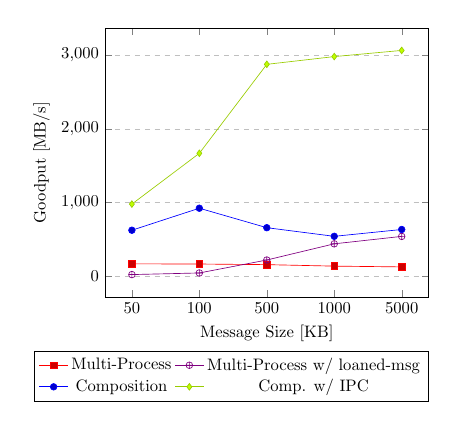
\begin{tikzpicture}[scale=0.60]
\begin{axis}[
    xtick=data,
    symbolic x coords={50, 100, 500, 1000, 5000},
    xlabel={Message Size [KB]},
    ylabel={Goodput [MB/s]},
    legend style={at={(0.39,-0.2)},anchor=north,legend columns=2},
    ymajorgrids=true,
    grid style=dashed,
    %log ticks with fixed point,
]
% Multi-Process
\addplot[red,every mark/.append style={solid,fill=red!80!black},mark=square*]
    coordinates {
    %(1, 12.13)
    (50, 167.74)
    (100, 165.3)
    (500, 156.77)
    (1000, 136.71)
    (5000, 126.13)
};
% Multi-Process SHM
\addplot[violet,every mark/.append style={solid,fill=violet!80!black},mark=oplus]
    coordinates {
    %(1, ???)
    (50, 21.97)
    (100, 43.94)
    (500, 219.72)
    (1000, 439.45)
    (5000, 540.18)
};
% Composition
\addplot[blue,every mark/.append style={fill=blue!80!black},mark=*]
    coordinates {
    %(1, 18.37)
    (50, 623.87)
    (100, 922.71)
    (500, 658.35)
    (1000, 541.17)
    (5000, 633.91)
};
% Composition IPC
\addplot[lime!80!black,every mark/.append style={fill=lime},mark=diamond*]
    coordinates {
    %(1, 23.38)
    (50, 978.51)
    (100, 1667.97)
    (500, 2875.57)
    (1000, 2980.60)
    (5000, 3064.31)
};
\legend{Multi-Process, Multi-Process w/ loaned-msg, Composition, Comp. w/ IPC}
\end{axis}
\end{tikzpicture}

\end{document}